<\chapter{Corriente de Saturación}
\section{Simulaciones}
\subsection{Simulacion(JFET)}


\begin{figure}[H]
    \centering

    \begin{minipage}{0.49\textwidth}
        \centering
        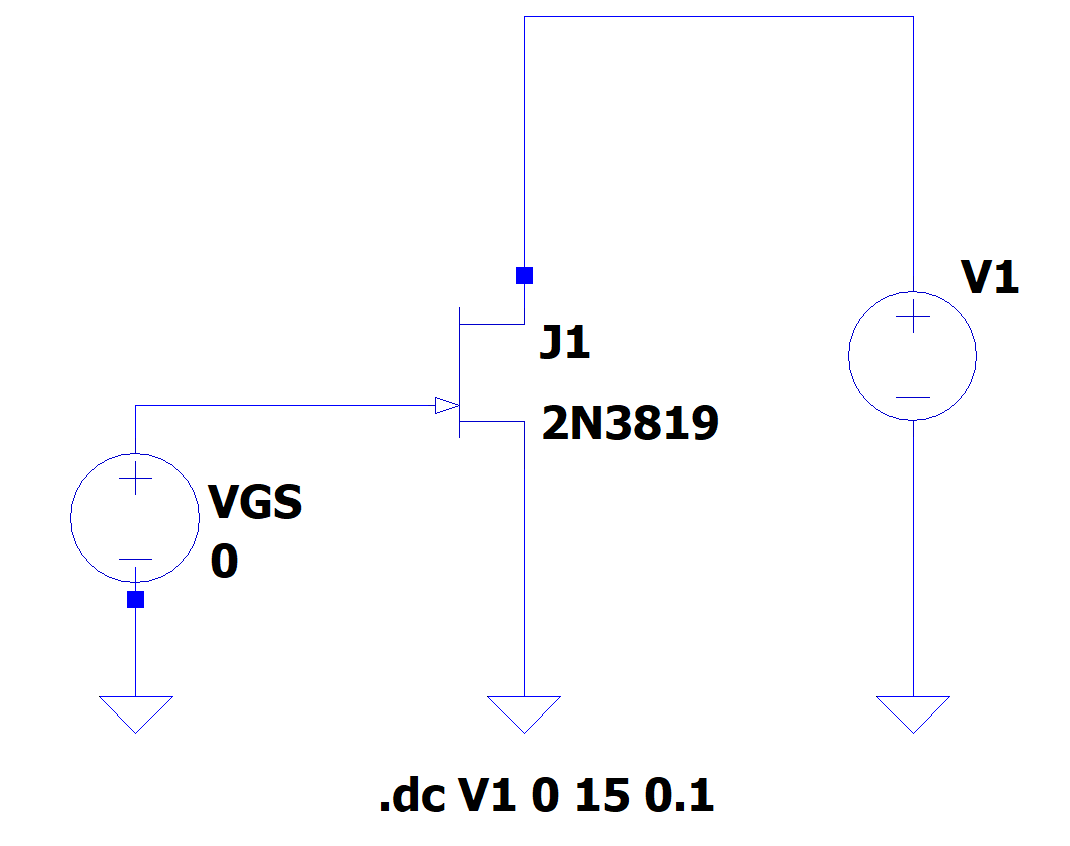
\includegraphics[width=\textwidth]{img/circuito_2N3819.png}
        \caption{Primera imagen}
    \end{minipage}
    \hfill
    \begin{minipage}{0.49\textwidth}
        \centering
        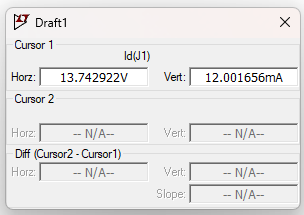
\includegraphics[width=\textwidth]{img/medicion_2N3819.png}
        \caption{Segunda imagen}
    \end{minipage}

\end{figure}





\begin{figure}[H]
\centering
\begin{tikzpicture}
\begin{axis}[
    width=16cm,
    height=9cm,
    ymin=-0.1,
    xmax=15.2,
    xmin=-0.1,
    xlabel={$V_1$ [V]},
    ylabel={$I_d$ [mA]},
    grid=major,
    minor tick num=1,
    grid=both,
]

\addplot[
    ultra thick,
    blue
]
table[
    col sep=tab,
    header=true,
    x index=0,
    y index=1,
    y expr=\thisrowno{1}*1000
] {dataTex/i(d)2N3819};
\addplot[
    only marks,
    mark=*,
    mark size=2.5pt
] coordinates {
    (13.6944,12)
}
node[
    above left
] {$I_{DSS}\approx12\,\mathrm{mA}$};

\end{axis}
\end{tikzpicture}
\caption{Curva del diodo 1N4007 en directa, obtenida por simulación}
\end{figure}



\begin{figure}[H]
    \centering
    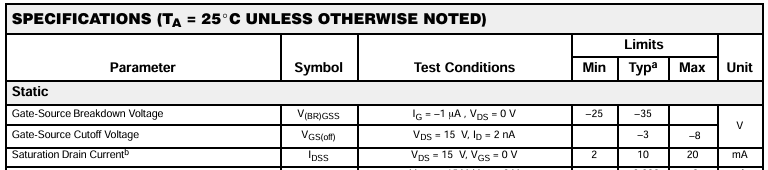
\includegraphics[width=\textwidth]{img/datasheet_2N3819.png}
    \caption{Descripción de la imagen.}
    \label{fig:imagen}
\end{figure}



\subsection{Simulación (MOSFET)}


\begin{figure}[H]
    \centering

    \begin{minipage}{0.49\textwidth}
        \centering
        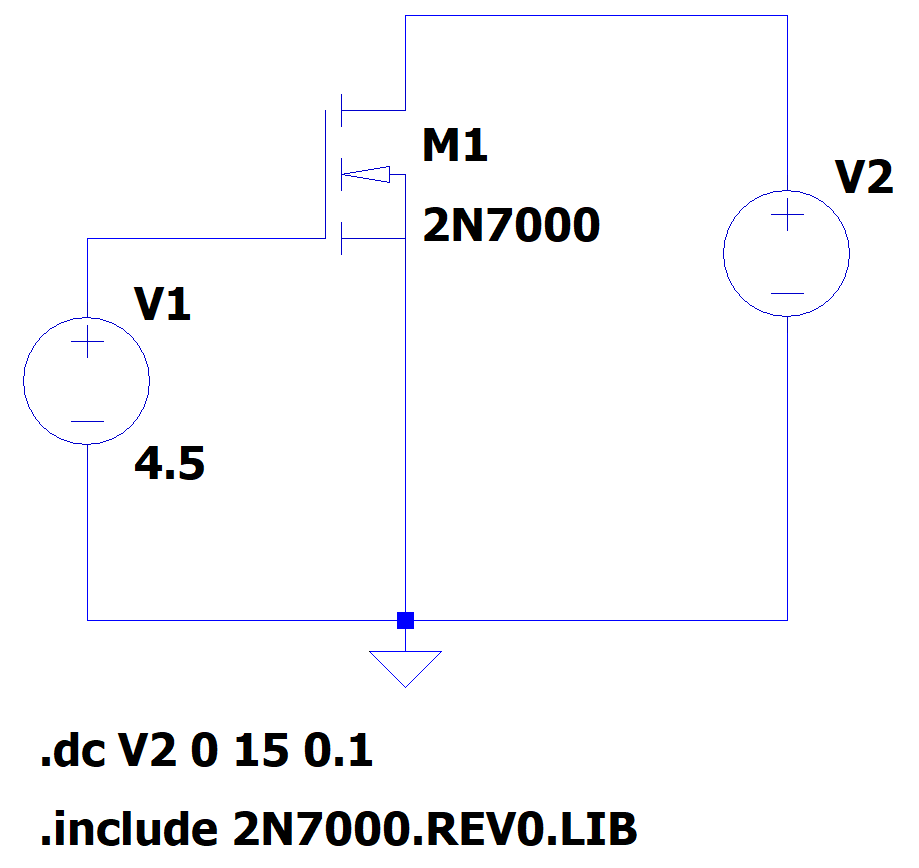
\includegraphics[width=\textwidth]{img/circuito_2N7000.png}
        \caption{Primera imagen}
    \end{minipage}
    \hfill
    \begin{minipage}{0.49\textwidth}
        \centering
        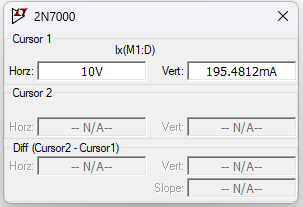
\includegraphics[width=\textwidth]{img/medicion_2N7000.png}
        \caption{Segunda imagen}
    \end{minipage}

\end{figure}


\begin{figure}[H]
\centering
\begin{tikzpicture}
\begin{axis}[
    width=16cm,
    height=9cm,
    ymin=-0.1,
    xmax=15.2,
    xmin=-0.1,
    xlabel={$V_{DS}$ [V]},
    ylabel={$I_d$ [mA]},
    grid=major,
    minor tick num=1,
    grid=both,
]

\addplot[
    ultra thick,
    red
]
table[
    col sep=tab,
    header=true,
    x index=0,
    y index=1,
    y expr=\thisrowno{1}*1000
] {dataTex/2N7000.txt};
\addplot[
    only marks,
    mark=*,
    mark size=2.5pt
] coordinates {
    (10,195.48)
}
node[
    above left
] {$I_{DSS}\approx195\,\mathrm{mA}$};

\end{axis}
\end{tikzpicture}
\caption{Curva del diodo 1N4007 en directa, obtenida por simulación}
\end{figure}


\section{Implementación en Laboratorio}



\begin{figure}[H]
    \centering
    \includegraphics[width=\textwidth]{img/Circuito_lab1.png}
    \caption{Descripción de la imagen.}
    \label{fig:imagen}
\end{figure}


\begin{table}[H]
\centering

\label{tab:valores_experimentales}

\begin{tabular}{|c|c|c|c|}
\hline
$V_{DS}$ [V] & $I_D$ [mA] & $V_{DS}$ [V] & $I_D$ [mA] \\ \hline
0,0  & & 8,0  & \\ \hline
1,0  & & 9,0  & \\ \hline
2,0  & & 10,0 & \\ \hline
3,0  & & 11,0 & \\ \hline
4,0  & & 12,0 & \\ \hline
5,0  & & 13,0 & \\ \hline
6,0  & & 14,0 & \\ \hline
7,0  & & 15,0 & \\ \hline
\end{tabular}

\caption{Valores experimentales de $I_D=f(V_{DS})$ para $V_{GS}=4,5\ \mathrm{V}$.}

\end{table}


\begin{figure}[H]
    \centering
    
    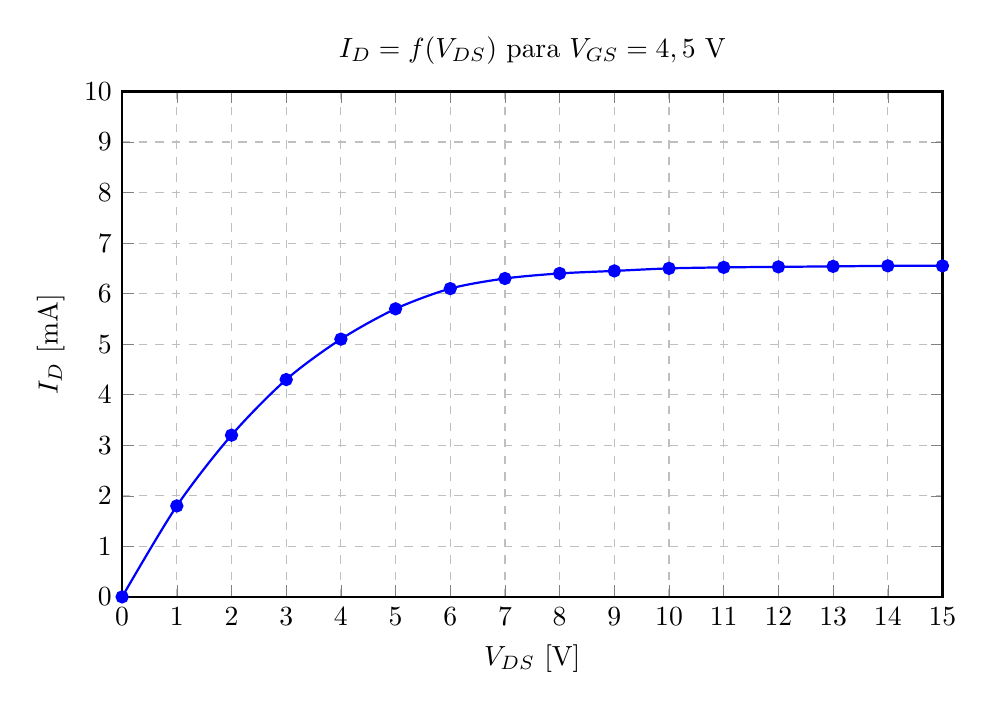
\begin{tikzpicture}
        \begin{axis}[
            width=12cm,
            height=8cm,
            xlabel={$V_{DS}$ [V]},
            ylabel={$I_D$ [mA]},
            title={$I_D=f(V_{DS})$ para $V_{GS}=4,5$ V},
            xmin=0, xmax=15,
            ymin=0, ymax=10,
            xtick={0,1,2,3,4,5,6,7,8,9,10,11,12,13,14,15},
            ytick={0,1,2,3,4,5,6,7,8,9,10},
            grid=both,
            minor grid style={dotted},
            major grid style={dashed},
            thick,
            mark size=2pt,
        ]
        
        \addplot[
            mark=*,
            smooth,
            thick,
            blue
        ] coordinates {
            (0,0)
            (1,1.8)
            (2,3.2)
            (3,4.3)
            (4,5.1)
            (5,5.7)
            (6,6.1)
            (7,6.3)
            (8,6.4)
            (9,6.45)
            (10,6.5)
            (11,6.52)
            (12,6.53)
            (13,6.54)
            (14,6.55)
            (15,6.55)
        };
        
        \end{axis}
    \end{tikzpicture}
    
    \caption{Curva experimental $I_D=f(V_{DS})$ para $V_{GS}=4,5$ V.}
    \label{fig:id_vds}
\end{figure}